\documentclass[english, 12pt]{beamer}
% Add handout to documentclass options if wanted

\usepackage[latin1]{inputenc}
\usepackage[T1]{fontenc}
\usepackage{babel,textcomp}


\usepackage{graphicx}
\usepackage{amsmath}
\usepackage{amssymb}
\usepackage{amsbsy}
\usepackage{amsfonts}
\usepackage{color}
\usepackage{xcolor}
\usepackage{epstopdf}
\usepackage{fancyvrb}
\usepackage{parskip}
\usepackage{url}
\usepackage{listings}

\DeclareMathAlphabet{\mathbfit}{OML}{cmm}{b}{it}

\definecolor{javared}{rgb}{0.6,0,0} % for strings
\definecolor{javagreen}{rgb}{0.25,0.5,0.35} % comments
\definecolor{javapurple}{rgb}{0.5,0,0.35} % keywords
\definecolor{javadocblue}{rgb}{0.25,0.35,0.75} % javadoc

\lstset{language=python,
basicstyle=\ttfamily\scriptsize,
keywordstyle=\color{javapurple},%\bfseries,
stringstyle=\color{javared},
commentstyle=\color{javagreen},
morecomment=[s][\color{javadocblue}]{/**}{*/},
% numbers=left,
% numberstyle=\tiny\color{black},
stepnumber=2,
numbersep=10pt,
tabsize=4,
showspaces=false,
captionpos=b,
showstringspaces=false,
frame= single,
breaklines=true}


\setlength{\arrayrulewidth}{1.6pt}
\renewcommand{\arraystretch}{1.2}
\newlength{\Tcalc}


\setbeamertemplate{frametitle}
{\begin{centering}\smallskip
\insertframetitle\par
\smallskip\end{centering}}
\setbeamertemplate{itemize item}{$\bullet$}
\setbeamertemplate{navigation symbols}{}
\setbeamertemplate{footline}[text line]{%
\hfill\strut{%
\scriptsize\sf\color{black!60}%
\quad\insertframenumber
   }%
    \hfill
}

% Define some colors:
\definecolor{DarkFern}{HTML}{407428}
\definecolor{DarkCharcoal}{HTML}{4D4944}
\colorlet{Fern}{DarkFern!85!white}
\colorlet{Charcoal}{DarkCharcoal!85!white}
\colorlet{LightCharcoal}{Charcoal!50!white}
\colorlet{AlertColor}{orange!70!black}
\colorlet{DarkRed}{red!70!black}
\colorlet{LightBlue}{blue!70!white}
\colorlet{DarkBlue}{blue!70!black}
\colorlet{DarkGreen}{green!70!black}

% Use the colors:
\setbeamercolor{title}{fg=Fern}
\setbeamercolor{frametitle}{fg=Fern}
\setbeamercolor{normal text}{fg=Charcoal}
\setbeamercolor{block title}{fg=black,bg=Fern!25!white}
\setbeamercolor{block body}{fg=black,bg=Fern!25!white}
\setbeamercolor{alerted text}{fg=AlertColor}
\setbeamercolor{itemize item}{fg=Charcoal}

\newcommand{\frn}[1]{\textcolor{Fern}{#1}}
\newcommand{\alrt}{\color{AlertColor}}
\newcommand{\bt}[1]{\textbf{#1}}
\newcommand{\kommando}[1]{\textcolor{AlertColor}{\texttt{\textbackslash #1}}}
\newcommand{\ds}{\displaystyle}

\renewcommand{\d}{\textrm{d}}

\title{Workshop: Projectile Motion \\ {\small An introduction to computing trajectories}}
\author{Jonas van den Brink \\ \texttt{j.v.brink@fys.uio.no}}
\institute{\alrt Simula Research Laboratory \\ Oslo, Norway}
\date{January 29, 2015}

\setbeamertemplate{frametitle}{\vspace{0.5cm} \insertframetitle} 

\begin{document}
\pagestyle{empty}

\begin{frame}
\maketitle 
\end{frame}

\begin{frame}
\frametitle{This workshop focuses on introducing computations to introductory physics}

Introducing computations should lead to a sense of empowerment

\vspace{1cm}

\visible<2-> {
For this to be possible, the computations must
\begin{enumerate}
	\item Relate to well-known problems
	\item Must be shown to be a powerful tool
	\item Understable. Students should write their own code
\end{enumerate}}
\end{frame}


\begin{frame}[fragile]
\frametitle{The goal is to find the velocity and position of an object as functions of time: $\vec{v}(t)$, $\vec{r}(t)$}

\begin{center}
\includegraphics[width=\textwidth]{fig/cannonball}
\end{center}

\visible<2->{	
Equations of motion
\begin{align*}
\alrt \frac{\d \vec{r}}{\d t} = \vec{v}(t), \qquad \frac{\d \vec{v}}{\d t} = \vec{a}(t)
\end{align*}}
\end{frame}

\begin{frame}[fragile]
\frametitle{The goal is to find the velocity and position of an object as functions of time: $\vec{v}(t)$, $\vec{r}(t)$}

Newtons 2.\ law of motion
$$\alrt \vec{F} = m\vec{a}$$

\visible<2->{	
\begin{center}
\includegraphics[width=\textwidth]{fig/cannonballforces}
\end{center}
}

\visible<3->{	
$$\alrt \vec{F}(r,v,t) = m\vec{a}(r,v,t).$$
}
\end{frame}

\begin{frame}[fragile]
\frametitle{The goal is to find the velocity and position of an object as functions of time: $\vec{v}(t)$, $\vec{r}(t)$}

Our algorithm is now as follows 

\begin{enumerate}
	\item Find the physical forces of the system.
	\item Use Newtons 2.\ law to find the acceleration
	\item Calculate $\vec{v}(t)$ and $\vec{r}(t)$ by solving the equations of motion
\end{enumerate}

\visible<2-> {
\vspace{1cm}
	In this workshop, we will solve step number 3 numerically, using the Euler method.
}



\end{frame}



\begin{frame}[fragile]
\begin{center}
{\Huge \color{DarkFern} The Euler Method}

\vspace{1cm}

A method for solving ordinary \\ differential equations (ODEs)
\end{center}
\end{frame}

\begin{frame}[fragile]
\frametitle{We can solve the equations of motion numerically using the Euler method}

\visible<2-> {	
From the definition of the derivative
\begin{align*}
\alrt \frac{\d v}{\d t} = \lim_{\Delta t \to 0} \frac{v(t+\Delta t) - v(t)}{\Delta t} =  a(t)
\end{align*}
}

\visible<3-> {
We now remove the limit, making $\Delta t$ a very small constant
\begin{align*}
\alrt \frac{v(t+\Delta t) - v(t)}{\Delta t} \approx  a(t)
\end{align*}
}

\visible<4-> {
Solving for $v(t+\Delta t)$ gives
\begin{align*}
\alrt v(t+\Delta t) \approx v(t) + a(t)\cdot \Delta t
\end{align*}
}
\end{frame}

\begin{frame}[fragile]
\frametitle{We can solve the equations of motion by stepping forward in time}

\begin{align*}
\alrt v(t+\Delta t) = v(t) + a(t)\cdot \Delta t
\end{align*}
\visible<2-> {	
If $a(t)$ and $v(t)$ are known, we can calculate $v(t+\Delta t)$
}

\visible<3-> {
\vspace{-0.2cm}
\begin{center}
\includegraphics[width=\textwidth]{fig/eulers0.pdf}
\end{center}
}
\end{frame}

\begin{frame}[fragile]
\frametitle{Our functions are no longer continuous, they have become discretized}

\visible<2-> {	
We only focus on multiples of our time-step
\begin{align*}
\alrt t & \alrt \in \{ 0,\ \Delta t,\  2\Delta t, \ 3\Delta t,  \ldots \} \\
\alrt t_i & \alrt \equiv i\cdot\Delta t
\end{align*}
}
\visible<3-> {	
Introduce the shorthand
\begin{align*}
\alrt v(t_i) &\alrt \equiv v_i \\
\alrt r(t_i) &\alrt \equiv r_i \\
\end{align*}
}

\visible<4-> {
 \vspace{-0.4cm}
\begin{center}
\includegraphics[width=\textwidth]{fig/time_discretization.pdf}
\end{center}
 \vspace{0.8cm}
}
\end{frame}

\begin{frame}[fragile]
\frametitle{We solve the equations of motion iteratively}

$$\alrt v_{i+1} = v_i + a_i\cdot\Delta t$$
\visible<2->{	
$$\alrt r_{i+1} = r_i + v_i\cdot \Delta t$$
}

\visible<3->{
For each time step, we must calculate the acceleration
$$\alrt a_i = a(r_i, v_i, t_i).$$
}

\visible<4->{	
We repeat these steps, starting at our initial conditions $v_0$ and $r_0$, until we have reached our end-time $t_N$
$$\alrt i = 0,1,2,3,\ldots, N.$$
}
\end{frame}

\begin{frame}[fragile]
\frametitle{Algorithm for the Euler method}

for $i=0,1,2,3,\ldots, N-1$:
\begin{enumerate}
	\item Use the previous results $x_i$ and $v_i$ to compute the acceleration: $\alrt a_i = F(x_i, v_i, t_i)/m$.
	\item Compute the new velocity: $\alrt v_{i+1} = v_i + a_i\Delta t$.
	\item Compute the new position: $\alrt r_{i+1} = r_i + v_i\Delta t$.
\end{enumerate}
\end{frame}


\begin{frame}[fragile]
\begin{center}
{\Huge \color{DarkFern} Implementation}

\vspace{1cm}

Moving from physics and math to \\ actual computer code
\end{center}
\end{frame}

\begin{frame}[fragile]

for $i=0,1,2,3,\ldots, N-1$:
\begin{enumerate}
	\item Use the previous results $x_i$ and $v_i$ to compute the acceleration: $\alrt a_i = F(x_i, v_i, t_i)/m$.
	\item Compute the new velocity: $\alrt v_{i+1} = v_i + a_i\Delta t$.
	\item Compute the new position: $\alrt r_{i+1} = r_i + v_i\Delta t$.
\end{enumerate}
\visible<2-> {
$$\Downarrow$$

\lstinputlisting{scripts/lsteuler.py}
}

\visible<3-> {
We want the code to look as much as possible like the physics and math we write on paper
$$\alrt t_i \Rightarrow \texttt{t[i]} \qquad  v_i \Rightarrow \texttt{v[i]} \qquad  r_i  \Rightarrow \texttt{r[i]}$$
}
\end{frame}

\begin{frame}[fragile]
\frametitle{We also need various bookeeping code}

Here we define the arrays we will be using
\lstinputlisting{scripts/lstarrays.py}
\end{frame}

\begin{frame}[fragile]
\frametitle{We also need various bookeeping code}

Here we define physical constants for our system and define the function that describes the forces

\lstinputlisting{scripts/lstforce.py}
This example show the forces acting on the cannonball as it sails through the air
$$\alrt F(x,v,t) = F_g + F_d(\vec{v}) = -mg\vec{k} - \frac{1}{2}\rho C_D A |\vec{v}|\vec{v}$$
\end{frame}

\begin{frame}[fragile]
\frametitle{As soon as we have solved the equations of motion, we can plot the result}

\lstinputlisting{scripts/lstplotting.py}
\end{frame}

\begin{frame}[fragile]
\begin{center}
	\includegraphics[width=\textwidth]{fig/plot_cannonball1}
\end{center}
\end{frame}

\begin{frame}
\begin{center}
{\Huge \color{DarkFern} Numerical Experimentation}

Altering parameters let's us immediately see the consequences
\end{center}
\end{frame}

\begin{frame}[fragile]
\begin{center}
	\includegraphics[width=\textwidth]{fig/plot_cannonball2}
\end{center}
\end{frame}

\begin{frame}[fragile]
\begin{center}
	\includegraphics[width=\textwidth]{fig/plot_cannonball3}
\end{center}
\end{frame}

\begin{frame}[fragile]
\frametitle{Students can use numerical experimentation to build intuition and knowledge}

\begin{itemize}
	\item Numerical results can be compared to known analytical solutions. Are numerical results trustworthy?
	\item Can study how results are directly changed by parameter choice. Are the parameters chosen reasonable?
	\item Can look at systems with and without certain contributions, such as air drag. \\ What is important, and what can be ignored?
\end{itemize}
\end{frame}

\begin{frame}
\begin{center}
{\Huge \color{DarkFern} Examples of possible projects}

You will have a chance to look at some of these today
\end{center}
\end{frame}

\begin{frame}[fragile]
\frametitle{Catapults and cannons and sports such as baseball}

\begin{center}
\includegraphics[width=\textwidth]{fig/cannonball}
\end{center}

\vspace{0.5cm}

\begin{itemize}
	\item Easy to compare with experimental data, either before or after simulation.
	\item Can look into studies of air drag, Reynolds number etc.
\end{itemize}
\end{frame}

\begin{frame}[fragile]
\frametitle{Skydiving and bungeejumping}

\begin{center}
\includegraphics[width=0.6\textwidth]{fig/skydiving}
\end{center}

\begin{itemize}
	\item Great study on free fall and terminal velocity
	\item Can study how parameters such as cross-sectional area and drag coefficient change as the parachute is opened
	\item Can plot the $g$-forces affecting the jumper. Which sport is more ``extreme''?
\end{itemize}
\end{frame}

\begin{frame}[fragile]
\frametitle{Pendulum and angular motion}

\begin{center}
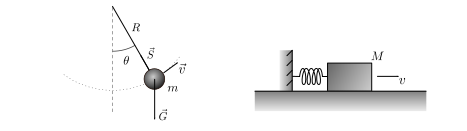
\includegraphics[width=\textwidth]{fig/pendulum}
\end{center}

\begin{itemize}
	\item Can solve pendulum also for large angles!
	\item Energy can be plotted as functions of time
	\item Can also simulate double pendulum and chaotic systems
\end{itemize}
\end{frame}

\begin{frame}[fragile]
\frametitle{Modelling the solar system}

\begin{center}
\includegraphics[width=0.4\textwidth]{fig/exopl_GJ1214b_ESO}
\end{center}

\begin{itemize}
	\item Students can gather real data of planetary orbits from NASA webpages
	\item Can combine numerical simulation with better graphics
\end{itemize}
\end{frame}


\end{document}